\begin{tiny}(Ega04)\end{tiny}
\begin{figure}[h!]
  \centering
  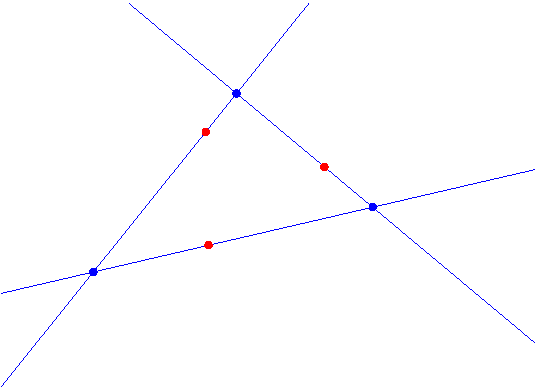
\includegraphics[width=7cm]{Ega04_1.pdf}
  % Egp11_1.pdf: 170x107 px, 72dpi, 6.00x3.77 cm, bb=0 0 170 107
  \caption{Exercice \arabic{enumi}: théorème de Ménéla{\"u}s.}
  \label{fig:Ega04_1}
\end{figure}

Les points $A$, $B$, $C$ d'un plan affine sont non alignés, les réels $\alpha$, $\beta$, $\gamma$ sont différents de $1$. Les points $L$, $M$, $N$ (voir figure \ref{fig:Ega04_1}) sont définis comme des barycentres de $A$, $B$, $C$ avec les coefficients suivants.
\begin{align*}
 L:(0,1,-\alpha) & & M:(-\beta, 0, 1) & & N:(1,-\gamma, 0)
\end{align*}
\begin{enumerate}
 \item Former une relation entre $\alpha$,$\beta$, $\gamma$ caractérisant l'alignement de $L$, $M$, $N$. Montrer que cette relation s'écrit
\begin{displaymath}
\frac{\overline{LB}}{\overline{LC}}\,
\frac{\overline{MC}}{\overline{MA}}\,
\frac{\overline{NA}}{\overline{NB}}=1 
\end{displaymath}
(théorème de Ménélaüs)
\footnote{voir la feuille \href{http://back.maquisdoc.net/data/temptex/fexgp.pdf}{Géométrie plane élémentaire}(exercices gp11.)}
\item Montrer que les droites $(A,L)$, $(B,M)$, $(C,N)$ sont concourantes ou alignées si et seulement si 
\begin{displaymath}
\frac{\overline{LB}}{\overline{LC}}\,
\frac{\overline{MC}}{\overline{MA}}\,
\frac{\overline{NA}}{\overline{NB}}=-1 
\end{displaymath}
(théorème de Céva)
\item Montrer que si $L$, $M$, $N$ sont alignés, les milieux des segments $AL$, $BM$, $CN$ sont alignés.\newline
On définit les points $L'$, $M'$, $N'$ comme des barycentres de $A$, $B$, $C$ avec les coefficients suivants.
\begin{align*}
 L':(0,-\alpha,1) & & M':(1, 0, -\beta) & & N':(-\gamma, 1, 0).
\end{align*}
Montrer que $L$, $M$, $N$ sont alignés si et seulement si $L'$, $M'$, $N'$ sont alignés. (les deux droites sont dites \emph{isotomiques})
\end{enumerate}
